% 04_framework.tex  --  WRITTEN
\section{The LA-JSSA Framework}
\label{sec:framework}

We now describe the two-timescale architecture that realizes the partially
observed control problem of Section~\ref{sec:system_model}. The design
separates a slowly-adapted supervised \emph{sensing tier}, which produces the
occupancy belief map $\belmap$, from a fast \emph{access tier} that learns the
policy $\pol$ by reinforcement~\cite{sutton2018rl}. Fig.~\ref{fig:arch} shows how the two tiers
close the sensing--access loop: the data flow
$\rx\to\spec\to\belmap\to\state\to\act$ feeds forward through the network,
and ACK/collision feedback from the environment returns to both the localizer
and the risk-constrained critic.

\begin{figure*}[t]
\centering
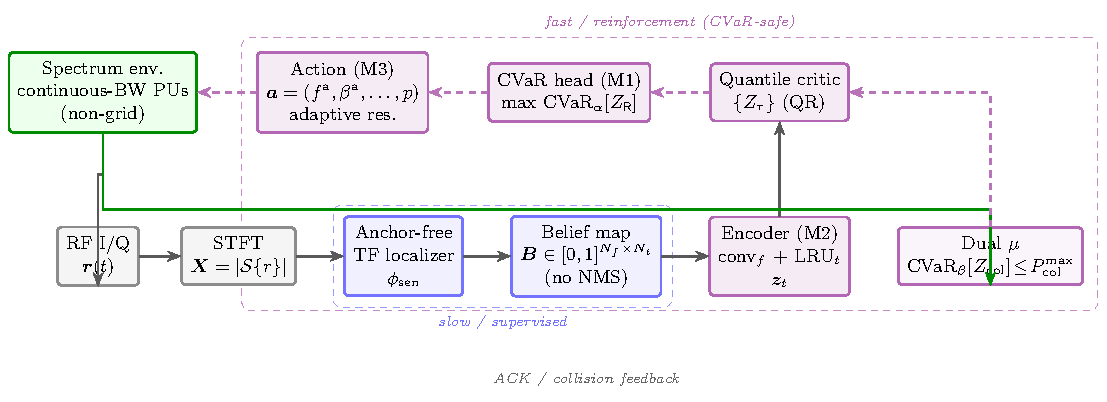
\includegraphics[width=0.95\textwidth]{figures/fig_arch.pdf}
\caption{The D-LA-JSSA two-timescale architecture. \emph{Bottom (slow,
supervised):} wideband in-phase/quadrature (I/Q) data are transformed to a spectrogram and passed to an
anchor-free TF localizer $\phi_{\mathrm{sen}}$ that emits a soft occupancy
belief map $\belmap$ (no NMS), encoded across time by a conv$_f$\,+\,LRU$_t$
encoder (M2). \emph{Top (fast, reinforcement):} a quantile critic feeds a
CVaR head (M1) and an adaptive-resolution action head (M3); a dual-ascent
multiplier enforces the CVaR collision constraint from ACK/collision
feedback. The environment of continuous-bandwidth, non-grid-aligned PUs
closes the loop.}
\label{fig:arch}
\end{figure*}

\subsection{Two-Timescale Rationale}
\label{subsec:twotimescale}
Joint end-to-end training of a detector and an RL agent is notoriously
unstable: the non-stationary reward signal corrupts the supervised gradient
of the detector, while a drifting detector keeps the RL state distribution
non-stationary. We therefore decouple the two. The sensing tier
$\phi_{\mathrm{sen}}$ is trained offline (or slowly online) on labeled
spectrograms with a supervised objective, so that the cell-level error rates
$\Pmd(\thr),\Pfa(\thr)$ of Assumption~\ref{as:cellerror} are stable; the
access tier then learns against an approximately stationary observation
channel. This mirrors the decoupled offline/online structure that is known
to accelerate partially observed Markov decision process (POMDP) learning
when the observation model is fixed.

\subsection{Sensing Tier: Belief-Map Generation}
\label{subsec:sensing_tier}
The sensing tier maps a spectrogram frame to the per-cell occupancy
posterior \eqref{eq:belief}. Because PU emissions have widely varying
time--frequency aspect ratios, we adopt an \emph{anchor-free} detector
(center/extent regression over the TF plane) rather than an anchor-based
region proposal network, which couples poorly to continuous, arbitrary
bandwidths~\cite{zhao2024uav}; when emissions overlap, a transformer backbone
that exploits TF correlation further improves
robustness~\cite{zhao2025trtfl_ssl}. The key departure from prior
TF-localization work is that we do \emph{not} apply NMS
to collapse the heatmap into hard boxes; instead the soft per-cell confidence
is retained as the belief map $\belmap\in[0,1]^{\Nf\times\Nt}$. This
preserves exactly the uncertainty that Theorem~\ref{thm:tradeoff} and the
reward \eqref{eq:reward} consume.

\begin{remark}[Design insight]
Discarding the soft confidence (the conventional detector output) is
information-lossy in the precise sense of Proposition~\ref{thm:sufficiency}: a
hard-box state is a deterministic coarsening of $\belmap$. The belief map is
an informative representation for the downstream access decision.
\end{remark}

\subsection{State Encoding Across Time (M2)}
\label{subsec:state_encoding}
To capture temporal correlation of PU activity under partial observability,
the access state \eqref{eq:state} stacks the most recent $\histlen$ belief
maps. The belief map is a two-dimensional TF object, so we encode it with a
\emph{factored} encoder: a convolution along the frequency axis captures the
spatial shape of emissions (their TF extent), while a point-wise linear
recurrent unit (LRU) along the time axis captures the long-range correlation
of PU on/off dynamics, producing a compact latent state
$\bm{z}_t = \mathrm{Enc}(\state_t)$. We adopt an LRU rather than a long
short-term memory (LSTM) network or a Transformer because recent evidence
shows point-wise recurrent state-space
models outperform attention on partially observable RL while remaining
parallelizable and lightweight~\cite{lu2024rethinking,morad2025cae}. The
recurrent encoding plays the role of the belief-update / sufficient-statistic
recursion of a POMDP. We ablate this choice (LRU vs.\ convolutional LSTM,
ConvLSTM) in Section~\ref{sec:simulation}.

\subsection{Access Tier: Continuous Resource Selection}
\label{subsec:access_tier}
The access tier maps the latent state to the resource-block action
\eqref{eq:action}. We consider two instantiations:
\begin{itemize}
\item a value-based agent over a discretized action grid (DQN~\cite{hausknecht2015drqn}
on $\bm{z}_t$), suitable when the TF action set is coarsely quantized; and
\item a continuous-control agent (deep deterministic policy gradient,
DDPG~\cite{lillicrap2016ddpg}) that
outputs $(\afc,\aBW,\ats,\adur,\pwr)$ directly, suitable for fine-grained
continuous resource selection.
\end{itemize}
Both optimize the constrained objective \eqref{eq:objective}; the
PU-protection constraint is enforced via a Lagrangian penalty whose
multiplier tracks the running collision rate against $\Pcolmax$.

\subsection{Distributional Safe Access (M1)}
\label{subsec:dist_rl}
Standard value-based agents learn only the expected return $\E[\Zret]$, which
discards exactly the information the belief map carries: the dispersion of
outcomes induced by occupancy uncertainty. We instead learn the full return
\emph{distribution} via a quantile critic, maintaining quantile estimates of
the throughput return $\Zthru$ and, separately, of the collision return
$\Zcol$. Two consequences follow.

First, the access objective becomes \emph{risk-sensitive}: rather than
$\max\E[\Zthru]$ we maximize a tail-aware utility
$\CVaR_{\cvarlvl}[\Zthru]$~\cite{rockafellar2000cvar}, which protects against rare low-throughput
episodes. Second, and more importantly for PU protection, the constraint is
imposed on the \emph{tail} of the collision-window return $\Zcol^{W}$ of
\eqref{eq:collision_window},
\begin{equation}
\max_{\pol}\;\CVaR_{\cvarlvl}\!\left[\Zthru\right]
\quad\text{s.t.}\quad
\CVaR_{\cvarcol}\!\left[\Zcol^{W}\right]\le\PcolmaxW,
\label{eq:cvar_objective}
\end{equation}
which is the formulation analyzed in Theorem~\ref{thm:cvar}. The CVaR terms
are estimated from the learned quantiles and the constraint is enforced by
dual ascent on a multiplier $\mu$ as in Algorithm~\ref{alg:lajssa}, with the
running windowed collision-CVaR estimate in place of the mean. By
Theorem~\ref{thm:cvar} the resulting operating point is at least as
conservative as the mean-constrained one, by a margin that vanishes as the
localizer sharpens---tying the method back to the value of TF localization.

\begin{remark}[Adaptive action resolution (M3)]
\label{rem:m3}
The quantile critic also exposes per-region uncertainty, which we use to make
the action resolution adaptive: in high-confidence idle regions the agent may
select a coarse, wide resource block, whereas near low-confidence boundaries
it is restricted to fine blocks. This couples the action granularity to the
belief entropy and is evaluated as an ablation in
Section~\ref{sec:simulation}.
\end{remark}

\subsection{Uncertainty-Aware Reward and Risk Sensitivity}
\label{subsec:reward_shaping}
The uncertainty term $\mathcal{U}(\belmap_t,\act_t)$ in the reward
\eqref{eq:reward} penalizes transmitting into TF cells whose occupancy
posterior is close to the undecided region. The following remark gives the
risk-sensitive reading of this penalty; it is an approximate justification,
not a strict equivalence.

\begin{remark}[Uncertainty penalty as a risk proxy]
\label{prop:risk}
Take $\mathcal{U}(\belmap_t,\act_t)=\sum_{\cell\in\mathcal{A}(\act_t)}
\bel_{m,n}(1-\bel_{m,n})$, the summed Bernoulli variance of occupancy over
the accessed cells. \emph{If} cell successes are conditionally independent
given $\belmap_t$ and the block throughput is linear in the per-cell
successes, then the conditional throughput variance is proportional to
$\mathcal{U}$, so $\E[\thru]-\lambda_{\mathrm{u}}\mathcal{U}$ approximates the
mean--variance criterion
$\E[\thru]-\tfrac{\lambda_{\mathrm{u}}}{2}\mathrm{Var}[\thru\mid\belmap_t]$
to second order, with $\lambda_{\mathrm{u}}$ playing the role of a
risk-aversion coefficient. Outside these conditions---correlated cells or
nonlinear reward---$\mathcal{U}$ should be read as an \emph{uncertainty
regularizer / risk proxy} rather than an exact variance, since it penalizes
undecided occupancy rather than interference variance directly.
\end{remark}

\noindent Read this way, the belief-map design is not ad hoc: the
uncertainty penalty steers the agent away from low-confidence cells, which
under the stated conditions coincides with risk-averse behavior. The full
procedure is summarized in Algorithm~\ref{alg:lajssa}.

\begin{algorithm}[t]
\caption{LA-JSSA training (one episode)}
\label{alg:lajssa}
\begin{algorithmic}[1]
\State \textbf{Input:} sensing net $\phi_{\mathrm{sen}}$ (pretrained),
threshold $\thr$, weights $\lambda_{\mathrm{c}},\lambda_{\mathrm{u}}$,
Lagrange multiplier $\mu$
\For{each frame $t$}
  \State acquire $\rx_t$; form spectrogram $\spec_t$ via \eqref{eq:stft}
  \State $\belmap_t \gets \phi_{\mathrm{sen}}(\spec_t)$
         \Comment{soft belief map, no NMS}
  \State $\state_t \gets (\belmap_{t-\histlen+1},\dots,\belmap_t)$;
         $\bm{z}_t \gets \mathrm{Enc}(\state_t)$
  \State select action $\act_t \sim \pol(\cdot\mid\bm{z}_t)$
         (DQN or DDPG head)
  \State transmit; observe ACK $\obs_t$ and collision indicator
  \State $r_t \gets \thru(\act_t) - \lambda_{\mathrm{c}}\mathrm{Col}(\act_t)
         - \lambda_{\mathrm{u}}\mathcal{U}(\belmap_t,\act_t)
         - \mu\,(\mathrm{Col}(\act_t)-\Pcolmax)$
  \State store $(\bm{z}_t,\act_t,r_t,\bm{z}_{t+1})$; update $\pol$
  \State $\mu \gets [\mu + \alpha_\mu(\widehat{\Pcol}-\Pcolmax)]_+$
         \Comment{dual ascent}
\EndFor
\end{algorithmic}
\end{algorithm}
